
\section*{Executive Summary}
\addcontentsline{toc}{section}{Executive Summary}

This report outlines the progress and achievements of the NGSOTI project,
aligning with the objectives and scope of the
\textbf{DIGITAL-2022-CYBER-B-03 — Cybersecurity and Trust} call \cite{EU2022CyberTrust}.
The project aims to support the market uptake and dissemination of innovative
cybersecurity solutions, with a particular focus on improving knowledge and
auditing cybersecurity preparedness across the EU.
The key outcomes and contributions of the project are as follows:

\begin{itemize}
    \item \textbf{Development of Training Infrastructure}: A state-of-the-art
training environment leveraging advanced technologies has been deployed to
enhance cybersecurity capabilities for SMEs, public organizations, and
educational institutions. The following advanced technologies were utilized:
\textbf{Headscale,LXC}. The NGSOTI project
aims to rely on \textbf{open-source technology} to ensure scalability, innovation,
and community collaboration. The following stakeholders used in 2024 NGSOTI,
SMEs, educational institutions.

    \item \textbf{Innovative Cybersecurity Solutions}: The NGSOTI platform has been instrumental in showcasing and utilizing innovative tools, including incident response solutions and cybersecurity investigation technologies, tailored to address real-world threats.

    \item \textbf{Market Readiness and Adoption}: By integrating cutting-edge
tools such as \textbf{Flowintel, MISP, Kunai and Tenzir} into its framework,
NGSOTI provides practical, market-ready solutions.These tools enable
organizations to enhance their resilience against cybersecurity threats.

    \item \textbf{Awareness and Education}: Training sessions and materials
have been delivered to a diverse audience, including SMEs, students, and professionals.
 
    \item \textbf{Community Engagement and Open Source}: The project actively
supports the open-source ecosystem through blog updates, the adoption of
collaborative tools, and dissemination activities. Most of tools in NGSOTI are open source.
This aligns with EU goals to improve the security of open-source ICT solutions.

    \item \textbf{Future-Focused Goals}: NGSOTI has contributed to advancing
cybersecurity preparedness by fostering the development of scalable, robust
solutions that address evolving regulatory and market needs, including
compliance with frameworks such as DORA and NIS2.
\end{itemize}

\subsection*{Advancing the Market-Readiness of Innovative Cybersecurity Tools}

As part of our commitment to fostering market-ready innovative cybersecurity 
solutions, \textbf{Kunai} has been successfully adopted by the
\textbf{Internet Storm Center (ISC)}\cite{kunai_isc_sans}, a division of the
SANS Institute. ISC operates as a global cybersecurity monitoring and analysis
center, known for its role in identifying and mitigating emerging threats.
By leveraging Kunai, ISC has enhanced its capabilities in analyzing and
processing malicious software, contributing to more robust threat intelligence
and incident response efforts.

Kunai's adoption by ISC underscores its readiness for real-world
cybersecurity applications and highlights its value in supporting critical
cybersecurity operations. This adoption represents a significant milestone in
our efforts to deliver impactful solutions that address complex cybersecurity
challenges at a global scale.

\chapter{NGSOTI Project: First-Year Status Overview}

This report provides an overview of the deployment status of the NGSOTI project,
focusing on the achievements of its key objectives. It highlights the progress
made and the impact of the implemented strategies on the project's success.
The document also reflects the collaborative efforts and innovations that have
driven the initiative forward, showcasing how the infrastructure and associated
goals align with the project's overarching mission.

Additionally, it details the deployment phase of the NGSOTI project, outlining
the steps taken to establish the project's infrastructure and ensure its
operational readiness. The report provides insights into the technical setup,
key components, and methodologies employed to achieve a scalable and robust
deployment. Furthermore, it highlights the challenges encountered during this
phase and the strategies implemented to address them, ensuring alignment with
the project's objectives and timelines.

The tables \ref{oa1}, \ref{oa2}, \ref{oa3}, \ref{oa4} compare the work package
objectives defined in the grant agreement with the achievements accomplished
so far. The first column identifies the work package number, prefixed by "WP"
followed by the number. The code "O" stands for "Objective," with the number
being a consecutive identifier derived from the grant agreement.
The next column describes the objective as defined in the grant agreement,
followed by a column indicating the state. States are represented as
follows: "O" for ongoing, "P" for pending, and "C" for closed. The subsequent
column summarizes the achievements, while the final column includes references
to chapters in the report for further details.

\begin{table}[h]
\centering

\begin{tabular}{ |p{0.07\linewidth}  |p{0.2\linewidth}|        p{0.04\linewidth}|    p{0.62\linewidth}|  p{0.07\linewidth}|}\hline
\multicolumn{5}{|p{0.97\linewidth}|}{Work Package 1} \\
\hline
                  Number             & Description & State & Achievements & Chapter \\
\hline
WP1.O1 &
A first objective is to ensure that the work defined in this project is executed in a timely matter & O &

The demand for training has exceeded initial projections, driven in part by
upcoming regulations such as DORA and NIS2, set to take effect in 2025.
The partial training infrastructure has been successfully
utilized in these sessions. While the increased demand for training was
successfully managed through the reallocation of resources, this did result
in some delays to project management tasks. We are actively addressing these
delays to ensure the project remains on track and aligned with our overall
objectives.
&
\ref{training}
 \\
\hline
WP1.O2 &
A second objective is that a smooth coordination between the partners is ensured
&O &
A real-time communication platform was established using Mattermost technology.
Monthly consortium meetings were held, subject to the availability of partners.
% Add achievements
&
%Add reference chapters
\\

\hline

WP1.O3 &
A third objective is that the necessary project management data is recorded
to ensure the reporting towards the funding
agency
& O &
In the first month, with the support of the project officer, the necessary
final documents were transmitted to the consortium to enable each partner to
evaluate what to expect during formal project reviews.
These topics were regularly discussed during consortium meetings.
&

\\

\hline

WP1.O4 &
A fourth objective is to set up the agreements to use NGSOTI for teaching
and research
& O &
A formal teaching agreement was signed with one institution, while two additional educational institutions joined the initiative in a less formal capacity. NGOSTI trainings are being delivered at these institutions, and they are also listed in the training section.
&
\ref{training}
\\

\hline
\end{tabular}
\caption{NGSOTI Objectives and Achievements Work Package 1}
\label{oa1}
\end{table}



\begin{table}[h]
\centering

\begin{tabular}{ |p{0.07\linewidth}  |p{0.2\linewidth}|        p{0.04\linewidth}|    p{0.62\linewidth}|  p{0.07\linewidth}|}\hline
\multicolumn{5}{|p{0.97\linewidth}|}{Work Package 2} \\
\hline
                  Number             & Description & State & Achievements & Chapter \\
\hline
WP2.O1 &
A first objective is to setup the technical infrastructure & O &

The NGSOTI project is a training infrastructure designed for security
operations training. It comprises three physical servers, datasets, and
auxiliary GPU-accelerated workloads. The virtual training environment is
built using LXC and Tailscale technologies, enabling the creation of
containers and a virtual network accessible from anywhere.

The infrastructure includes components such as Headscale for authentication
and Access Control Lists. Documentation is also provided. Hardware
procurement was completed, and the equipment was set up to establish a
phishing platform for training activities. Dataset processing has been
initiated.

&
2,3 \\
\hline
WP2.O2 &
A second objective to maintain the infrastructure agile to easily adapt to new
SOC paradigms
&O &
Two types of adaptations have already been demonstrated:
\begin{itemize}
    \item \textbf{Incremental Design}: The training infrastructure was made
    operational and ready for use, even though it was not yet fully deployed.
    \item \textbf{Adoption of New Tools}: Tools such as Flowintel were introduced
    for case management, replacing RT, and Tenzir was adopted as an alternative
    to Zeek.
\end{itemize}

&
%Add reference chapters
\\

\hline

WP2.O3 &
A third objective collect data of the infrastructure
& O &
During the first year of the project, over 4 TB of network traffic capture data was collected and presented at two conferences. Additionally, a Linux malware dataset was compiled and published.
&
% Add reference chapters
%TODO add reference to https://helga.circl.lu/NGSOTI/malware-dataset
\\

\hline

WP2.O4 &
An independent satellite task will be the URL checker for the Restena edu.lu
service including a malicious link report
option
& P &
% Add achievements
&
%Add reference chapters
\\
\hline
\end{tabular}
\caption{NGSOTI Objectives and Achievements Work Package 2}
\label{oa2}
\end{table}


\begin{table}
    \begin{tabular}{ |p{0.07\linewidth}  |p{0.2\linewidth}| p{0.04\linewidth}| p{0.62\linewidth}|  p{0.07\linewidth}| }
    \hline
    \multicolumn{5}{|p{0.97\linewidth}|}{Work Package 3} \\
    \hline
    Number & Description & State & Achievements & Chapter \\
    \hline
    WP3.O1 & Evaluate the data of NGSOTI to create up-to-date training materials & O & Training materials are being updated based on analyzed data & \\
    \hline
    WP3.O2 & Perform training with NGSOTI & O &  More training sessions than initially expected were successfully delivered using NGSOTI. &  \\
    \hline
    WP3.O3 & Collect feedback from existing trainings to improve future ones & O & Feedback has been gathered and is being analyzed for implementation &  \\
    \hline
    \end{tabular}
    \caption{NGSOTI Objectives and Achievements Work Package 3}
\label{oa3}
\end{table}


\begin{table}
        \begin{tabular}{ |p{0.07\linewidth}  |p{0.2\linewidth}| p{0.04\linewidth}| p{0.62\linewidth}|  p{0.07\linewidth}| }
        \hline
        \multicolumn{5}{|p{0.97\linewidth}|}{Work Package 4} \\
        \hline
        Number & Description & State & Achievements & Chapter \\
        \hline
        WP4.O1 & Make NGSOTI attractive for schools and students & O &NGSOTI was
        utilized for engineering as well as bachelor’s and master’s students.
        Additionally, it garnered interest from security professionals and open-source
        enthusiasts, where it was successfully demonstrated.  & 1 \\
        \hline
        WP4.O2 & Enable teachers to use NGSOTI to create training materials & O &
        The NGSOTI infrastructure was demonstrated during a MISP training session for
        students, and its functionality was explained to teachers. & 2 \\
        \hline
        WP4.O3 & Maintain blog posts about the components used within NGSOTI & O &
        Blog posts published, keeping the community informed about updates &  \\
        \hline
        \end{tabular}
    \caption{NGSOTI Objectives and Achievements Work Package 4}
    \label{oa4}
\end{table}





\chapter{Deployment Status}

In the NGSOTI project, the consortium closely monitored the behavior and requirements of its user communities, ensuring the development and customization of tools tailored to support efficient Security Operations Center (SOC) operations. These tools are detailed in the following section.

\section{Optimized Tools for Streamlined SOC Operations}

\subsection{Tenzir}

Tenzir is an open-core data pipeline management (DPM) tool that enables security
teams to collect, normalize, enrich, and route security data. NGSOTI relies on
Tenzir for automating the exchange of event data between various tools, such as
Kunai, MISP, and OpenSearch. In addition to data integration, Tenzir executes
detection content in the pipeline with its enrichment framework and built-in
operators to execute Sigma and YARA rules. These features are a central reason
for using Tenzir within NGSOTI, as they are not available in general-purpose
data pipeline tools, such as Fluent Bit.

\subsubsection{Use Cases}

For NGSOTI, Tenzir specifically supports the following use cases:

\begin{itemize}
\item \textbf{Kunai Log Collection}: Tenzir picks up Kunai log files and ships
	them to a central location. Kunai writes its logs as JSON to a file,
	which Tenzir can pick up, parse, and normalize.
\item \textbf{OCSF Event Normalization}: Tenzir is purpose-built to map security
	telemetry from disparate sources in various formats to a canonical form
	for easier correlation. The Open Cybersecurity Schema Framework (OCSF)
	is the de-factor standard for security teams and has been adopted by
	Linux Foundation in late 2024. Tenzir makes it easy to transform events
	to OCSF and also add OCSF-compliant enrichment objects in its pipelines.
\item \textbf{MISP Content Operationalization}: Tenzir can operationalize MISP
	events and contained attributes by making the data available in
	pipelines to flag sightings. The reported sightings do not only serve as
	corroborating evidence in the subsequent alert processing, but also
	deliver valuable threat insights when sent back to MISP.
\end{itemize}

\subsubsection{Key Activities}

In 2024, Tenzir focused on building key capabilities that enable the above
mentioned use cases within the NGSOTI project.

\begin{itemize}
\item \textbf{Tutorial on OCSF Normalization}: To teach SOC operators how to
	standardize event data for subsequent analytics across multiple data
	sources, Tenzir published a tutorial that outlines the key steps in
	great
	detail\cite{tenzir_ocsf_tutorial}.

\item \textbf{Lookup Table Aggregations}: Tenzir's lookup tables are a building
	block for several SecOps use cases. In addition to using them for
	enriching event streams with indicators of compromise that arrive from
	MISP, they can be used to passively collect observed data for subsequent
	enrichment.

	This is particularly useful for building a passive inventory of assets.
	A popular example involves computing first/last/times-seen statistics to
	build passive DNS tables. But also extracting IP-to-MAC,
	host-to-username, or any other mappings available in telemetry provide
	valuable context for entity-based reasoning.

	Tenzir presented this feature along with various examples at Suricon
	in November
	2024.\cite{suricata_meets_ocsf}

\item \textbf{OpenSearch/ElasticSearch and Splunk Support}: SOC operators often
	use a SIEM to analyze logs centrally. Since the mission of NGSOTI is to
	prepare the next generation of SOC operators for real-world settings
	where they will likely encounter a SIEM, Tenzir built native
	integrations for the most commonly used SIEMs out there:
	OpenSearch/ElasticSearch (via the Bulk API) as well as Splunk.

\item \textbf{String Function Processing}: In order to support flexible
	dissection of string data that comes—among other tools—from MISP, Tenzir
	added numerous functions for native string inspection and
	transformation\cite{tenzir_tql2_string_functions}.

	These functions are building block for the MISP integration, which
	requires receiving data via ZeroMQ, splitting strings at a space, and
	then parsing the second component as JSON. Tenzir now has all of these
	building blocks in place to trivially support reading data in real time
	from MISP in a structured manner.

\item \textbf{Community ID Computation}: In order t correlate network with
	endpoint events, Tenzir added a function to compute the Community ID of
	a network
	flow\cite{tenzir_community_ids}.

	Kunai also added a feature to support Community ID computation, making
	it now possible to correlate network data from Zeek and Suricata with
	Kunai in Tenzir.
\end{itemize}

In summary, Tenzir added essential capabilities for SOC operators that seek to
integreate various security tools and their dataflows.

\subsection{SkillAegis}
SkillAegis is an excellent outcome of the NGSOTI project, aligning seamlessly with its mission to train the next generation of SOC operators. While the project emphasizes creating operational infrastructures and fostering hands-on training environments, SkillAegis addresses the critical human element by providing a platform for scenario-based training.
SkillAegis equips trainees with practical skills to navigate these challenges by simulating real-world incidents in a controlled, dynamic environment.
This tool complements the project's vision by enhancing traditional training methods, including academic curricula and industry-led guest lectures, with interactive, real-data-driven cyber range exercises. Hosted by CIRCL and supported by Restena's network interconnectivity, the infrastructure enables SkillAegis to play a pivotal role in preparing SOC operators for future challenges while fostering a collaborative and robust educational ecosystem.

On August 14, 2024, the release of \textbf{SkillAegis v1.0.0} was announced on misp-project.org. SkillAegis is an open-source platform developed as part of the NGSOTI project to advance cybersecurity training and capacity building. SkillAegis is designed to enhance cyber threat intelligence training through realistic, scenario-based exercises, enabling participants to simulate and respond to real-world cyber incidents.

\subsubsection{Key Features of SkillAegis}
\begin{itemize}
	\item \textbf{Scenario Creation:} Trainers can design customized exercises with specific learning objectives, simulating various cyber incidents to develop practical skills in threat intelligence and information management.
	\item \textbf{Exercise Execution \& Monitoring:} The platform allows trainers to deploy and oversee scenarios in real-time, using a live dashboard to track participant progress and provide immediate feedback.
\end{itemize}

\subsubsection{Components of the SkillAegis Platform}
\begin{itemize}
	\item \textbf{SkillAegis Main Application:} Serves as the core component, managing scenario execution and integrating ready-to-use training modules.
	\item \textbf{SkillAegis Editor:} Enables trainers to create new exercises, including metadata, injects (tasks), execution order, and evaluation criteria. It also features an Inject Tester to optimize scenarios.
	\item \textbf{SkillAegis Dashboard:} Facilitates training session execution and provides real-time insights into participant progress, including completion status and logs of user actions.
\end{itemize}

\subsubsection{Integration with MISP}
SkillAegis was specifically developed to integrate with MISP (Threat Sharing Platform), enhancing training quality. Injects can directly interact with data within MISP, querying and monitoring user activity. To enable this, SkillAegis connects to a training MISP instance via a valid site-admin API (Application Programming Interface) Key.

\subsubsection{Availability and Licensing}
SkillAegis is freely available as open-source software under the AGPLv3 license, reflecting its EU project origins and commitment to supporting the cybersecurity community. The platform can be downloaded and utilized at no cost.

For more information and access to SkillAegis, visit the \href{https://www.misp-project.org/2024/08/14/SkillAegis-v1.0.0.html/}{official announcement}.


\subsection{MISP Training Infrastructure}
MISP is a core element of the NGSOTI infrastructure, and stakeholders often request dedicated MISP training sessions. Since MISP is a fully distributed system, participants should be able to explore and experiment with data flow aspects. To facilitate this, a network of temporary MISP servers was set up for training purposes. These seven servers are publicly accessible, allowing participants to configure synchronization rules as needed. The deployment of the servers was fully automated, including their configuration with default user accounts for participants. After each training session, the servers are reset to provide new trainees with a clean environment. The deployment is managed using LXC technology. LXC (Linux Containers) is a lightweight virtualization technology that enables the creation of isolated environments on a single host by sharing the host's Linux kernel. Unlike traditional virtual machines, LXC containers are more resource-efficient and faster to start, as they don't require a separate operating system. They are ideal for use cases such as development, testing, training, and multi-tenancy, providing secure isolation and flexible resource management through namespaces and cgroups.


\subsection{Kunai}

While Linux workstations may not rival Windows or macOS systems in popularity, Linux systems dominate the server landscape, often hosting critical services such as web servers, databases, and many public systems accessible via the Internet. However, Linux security monitoring for SOCs frequently lacks the detailed visibility available on Windows systems, where free tools like Sysmon\cite{sysmon_tool} exist. SOC engineers often rely on audit logs or application logs to create detection scenarios, but these sources are not always security-focused and typically lack correlation capabilities necessary for understanding the occurrence of suspicious events.

An attempt to port Microsoft Sysmon to Linux was made\cite{sysmon_linux}.
However, the project suffers from several Linux-specific design flaws and has
not seen maintenance since its release, making it unappealing for potential
users. Other projects, such as
\textbf{Tracee}\cite{tracee_aquasecurity}
and \textbf{Falco}\cite{falco_falcosecurity},
address Linux security visibility issues but lack some key features offered by Sysmon,
including threat-hunting capabilities and event correlation for root cause analysis.

From our experience, alert contextualization and root cause analysis are
crucial for enabling SOC operators to triage alerts effectively and for
incident responders to thoroughly investigate security events. These needs
motivated the development of \textbf{Kunai}, with the goal of providing a
tailored security visibility tool for Linux systems. Kunai empowers SOC
engineers and incident responders to perform their jobs more effectively and
efficiently.

As part of the \textbf{NGSOTI} project, Kunai has undergone significant
enhancements to achieve its goals. Integration with
\textbf{MISP}\cite{misp_project}
enables Kunai to leverage Indicators of Compromise (IOCs) and threat intelligence
shared through the platform. This fosters community-based intelligence sharing
and simplifies the detection of known threats. Additionally, a rule engine was
developed to facilitate log filtering and the creation of highly customizable
detection rules tailored to specific needs and environments. The rule format was
designed to be simple to write and share, promoting collaboration and distribution
through platforms like \textbf{MISP}. These contributions make data sharing
among SOCs seamless, allowing incidents to be detected and addressed more quickly.

Some of the other contributions made under \textbf{NGSOTI} include:
\begin{itemize}
	\item Integration of numerous new security events, providing enhanced
visibility, analysis, and detection capabilities.
	\item File scanning using
\textbf{Yara}\cite{yara_x} rules for malicious file detection.
	\item \textbf{Community-ID}\cite{community_id_spec}
support, enabling correlation between system logs and network logs from tools
like \textbf{Suricata}\cite{suricata_website}
and \textbf{Zeek}\cite{zeek_website}.
\end{itemize}

Finally, several production-readiness features have been implemented, such as
automated installation and configuration and log rotation. Background tasks
such as maintaining an up-to-date website and documentation\cite{kunai_why},
monitoring Linux kernel changes to reflect in the project, and refactoring
code have also been undertaken to ensure the project's long-term reliability
and relevance.

\subsection{Vulnerability Lookup}
Effective vulnerability management is a critical aspect of SOC operations,
requiring the ability to handle and prioritize vulnerabilities efficiently.
Historically, only a few vulnerability databases existed, but with the
introduction of the NIS2 directive promoting enhanced vulnerability management,
the number of databases has grown significantly. This proliferation poses
challenges for SOC operators in reconciling and aggregating data across
multiple sources. To address this, NGSOTI extended and integrated the
open-source tool Vulnerability Lookup\cite{vulnerability_lookup},
streamlining the process and improving operational efficiency.

\textbf{Vulnerability-Lookup} is an open-source tool that facilitates the correlation 
of vulnerabilities from various sources, independent of their IDs, and streamlines 
Coordinated Vulnerability Disclosure (CVD) management. It serves as a collaborative 
platform where users can comment on security advisories, create bundles, and add 
observations. An instance operated by CIRCL is available at 
\url{https://vulnerability.circl.lu}.

\textbf{Key Features:}
Vulnerability-Lookup provides a comprehensive API for fast vulnerability searches, 
a modular feeder system for importing vulnerabilities from sources like CISA, NIST, 
GitHub, and OpenSSF, and supports creating and editing Security Advisories with the 
vulnogram editor. Users can add sightings (e.g., seen, exploited, patched) to 
vulnerabilities, share comments, and create bundles of advisories. Integration with 
EPSS and extensive RSS/Atom feeds are also included.

\textbf{Sighting Sources:}
It supports various sighting sources, including Fediverse, MISP, Nuclei, Exploit-DB, 
CISA KEV, and RSS. Users can also create custom sighting tools using the 
\texttt{PyVulnerabilityLookup} library.

\textbf{Installation:}
Vulnerability-Lookup requires Python 3.10, Poetry, and a Kvrocks database. Detailed 
installation instructions and architecture are provided in the official documentation.


\section{NGSOTI Core Infrastructure}

Both partners LHC and Restena procured hardware to support the project. Restena's
hardware is used for processing activities, such as handling Blackhole data.
They set up the equipment in the data center and initiated the first
processing of the Blackhole data. Additionally, Restena established a
phishing platform to create phishing campaigns as part of the training
activities. LHC's hardware was also deployed in a data center and serves as
the core infrastructure for NGSOTI, ensuring the project's operational foundation.

As depicted on~\ref{fig1}, {\bf{ngsoti1}} holds a headscale LXC container to
manage the authentication of users, and Access Control Lists. Within the LXC
virtual network, there is a special LXC container that is also part of the
tailscale VPN (the tailnet) that acts as a router to the virtual training
infrastructure.

NGSOTI Core Infrastructure encompasses the software stack that is used for
hosting the services and datasets that trainees and trainers have access to
within the framework of the action.

\begin{itemize}
	\item {\bf{ngsoti1}} is a physical server that hosts LXC containers and that host the virtual training network,
	\item {\bf{ngsoti2}} is a physical server that hosts the datasets used during training (e.g. collections from the blackhole, malware samples, etc.)
	\item {\bf{ngsoti3}} is a physical server that host auxiliary GPU accelarated workloads (e.g. A.I webservices)
\end{itemize}



\begin{figure}[ht]
	\centering
	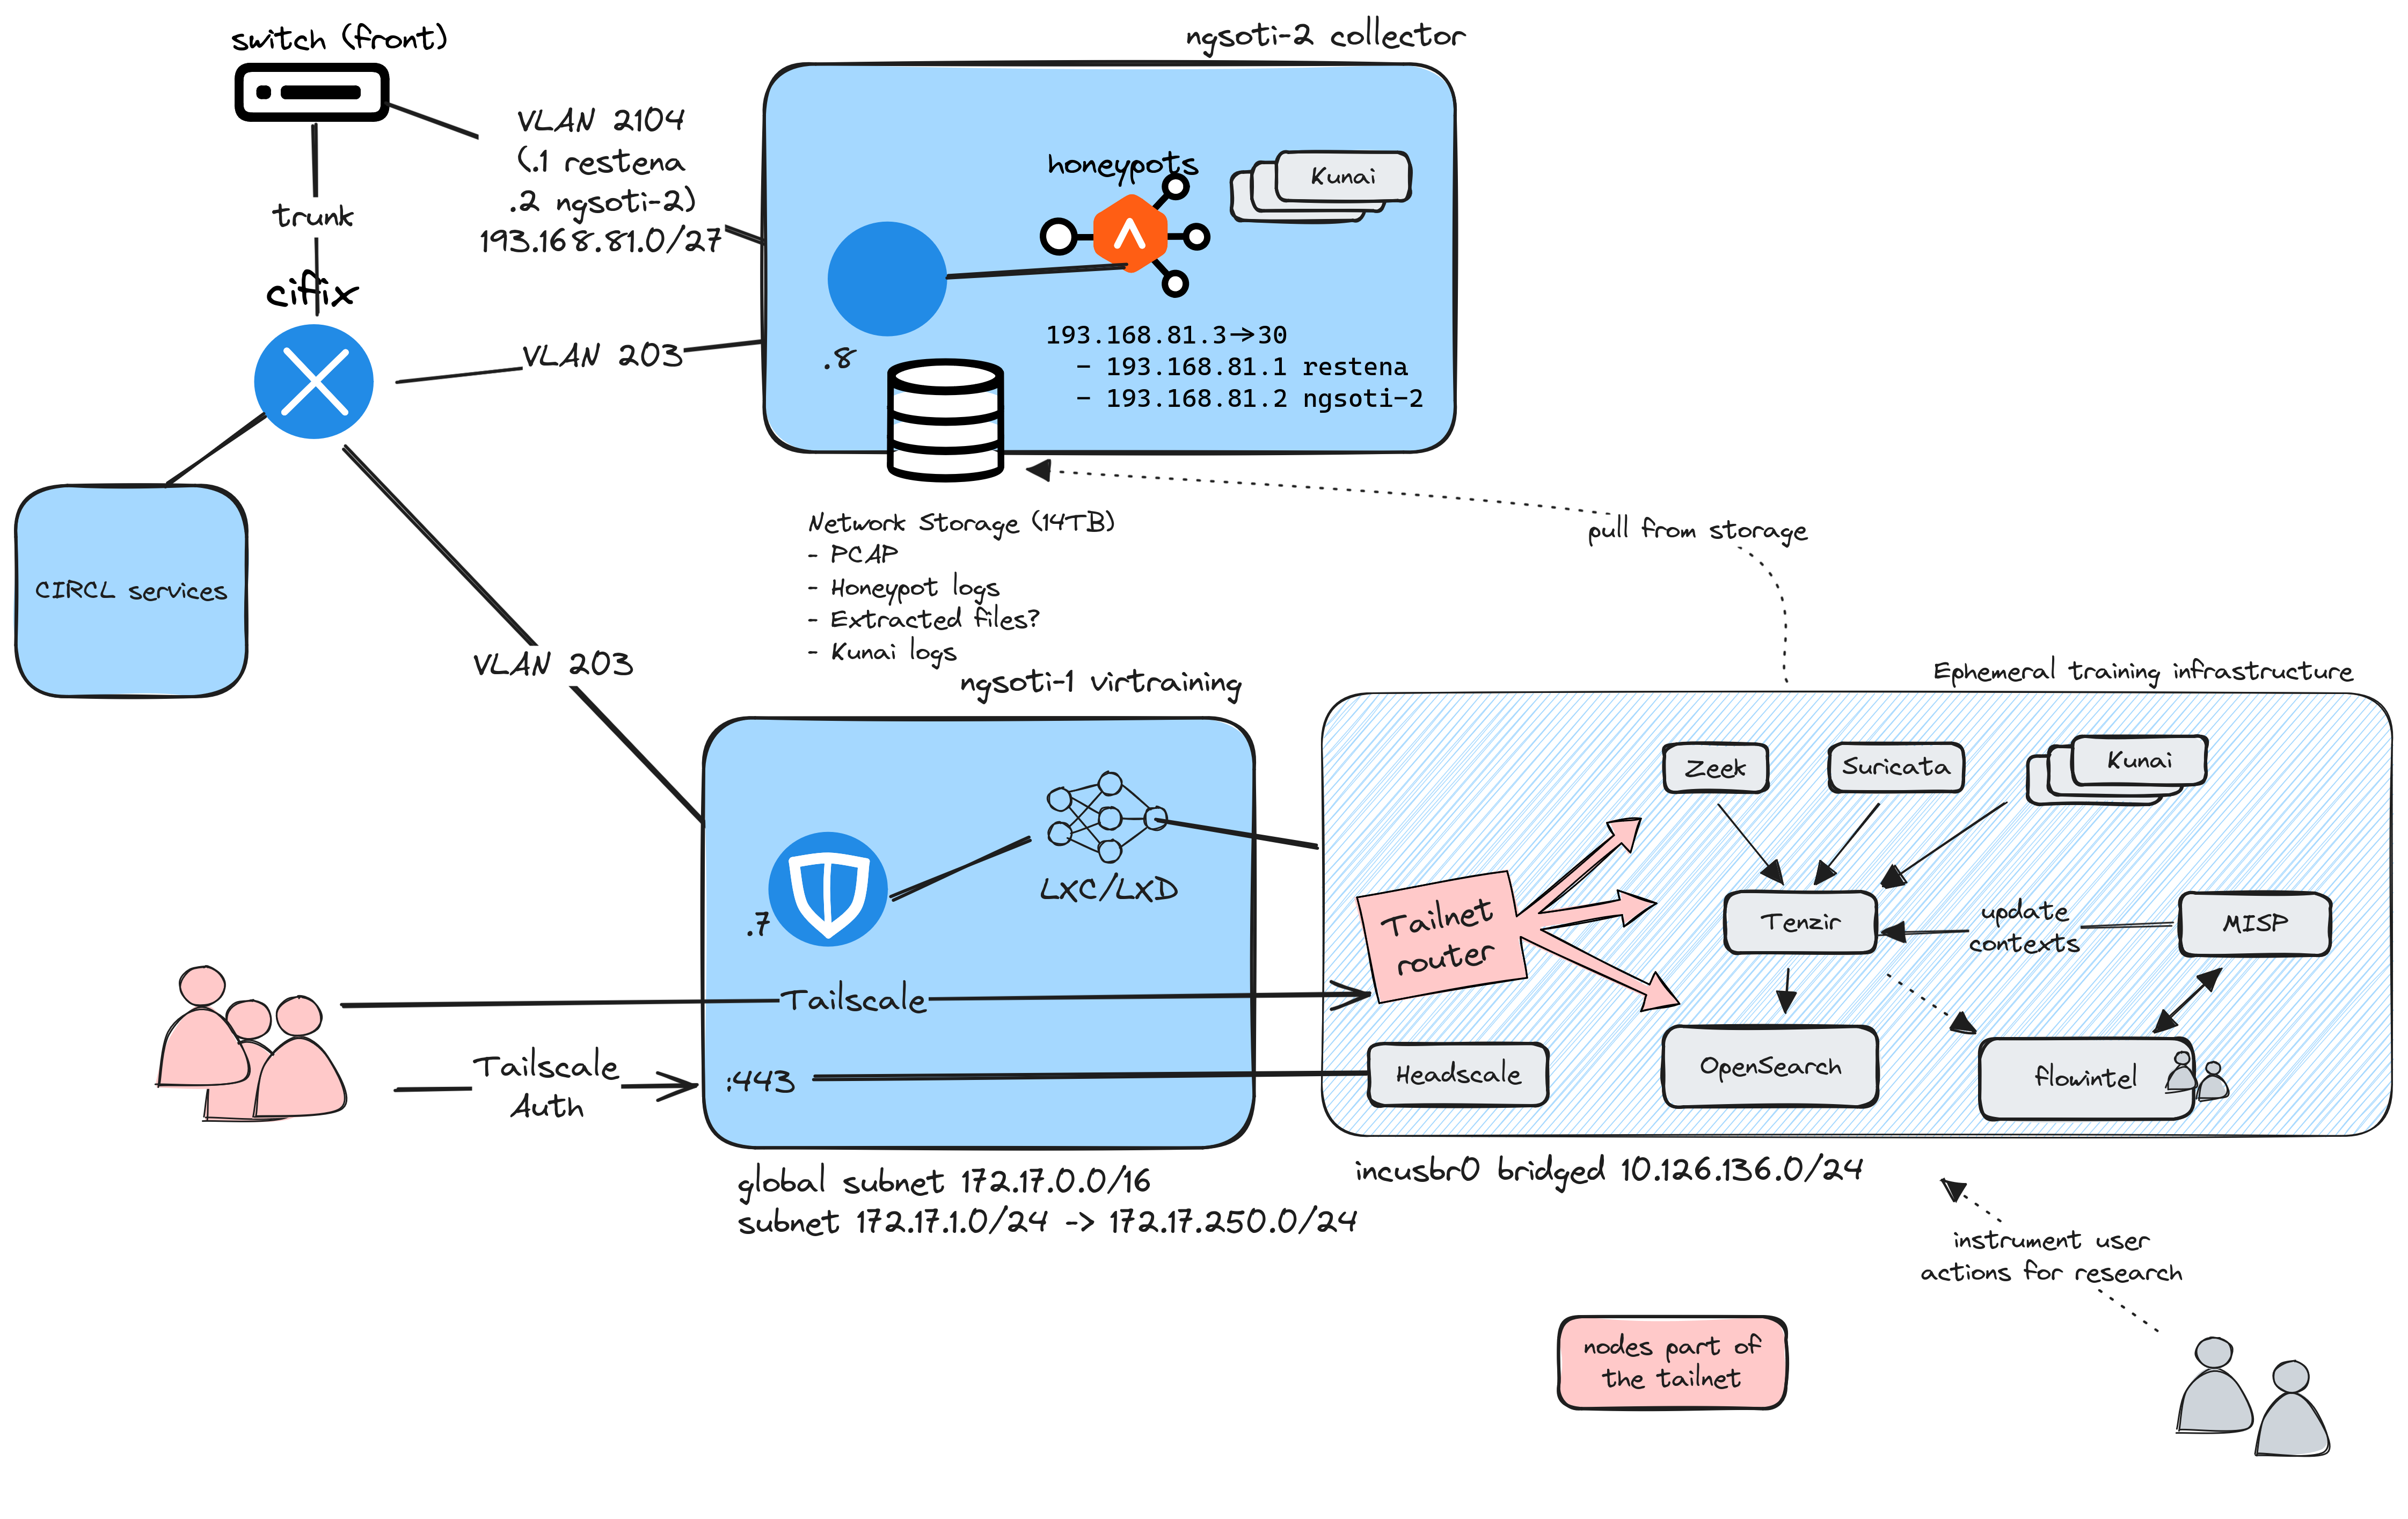
\includegraphics[width=\textwidth]{./img/NGSOTI-architecture.png}
	\caption{NGSOTI core infrastructure diagram}
	\label{fig1}
	\end{figure}

The virtual training environment hosted on {\bf{ngsoti1}} is built around two main pieces of technology:

\begin{itemize}

	\item {\bf{LXC}} is a container runtime for
	linux\cite{linux_containers}. It allows for the
	creation of containers holding the differents services used during
	trainings, as well as for the creation of a virtual network that users will
	use to connect to the differents services. The LXC infrastructure offers
	profiles that can be applied on newly created containers to easily create
	SSH admin access, and mount datasets from {\bf{ngsoti2}}
	
	\item {\bf{tailscale}}\cite{tailscale,} is a VPN
	(Virtual Private Network) technology that allows us to give access to the
	virtual network from anywhere where the tailscale client can run. In
	addition to tailscale, we run
	{\bf{headscale}}\cite{headscale} that is an open
	source project used to manage tailscale authentication.
	
\end{itemize}

The virtual training infrastructure is accessible to trainers, trainees, and
administrators through the tailnet. Comprehensive documentation is available
to support their use of the platform. The documentation is organized into
distinct segments for each component, ensuring clarity and ease of reference.

\begin{description}
	\item [overall architecture] Tailscale is a mesh VPN built on WireGuard,
enabling secure, private networking within a tailnet. In this setup, a custom
coordination server replaces the default
Tailscale servers, providing greater control and privacy. Users authenticate
using a reusable, non-expiring pre-authentication key and gain access to a
tailnet-router container that routes traffic to LXC containers hosted on the
server. After downloading the Tailscale client and connecting with the
provided configuration, users can securely access resources within the
tailnet, such as SSH into containers, provided their SSH key is authorized.
This setup ensures efficient and private access to network resources.
	\item [how to create containers]
Headscale is a self-hosted implementation of Tailscale's coordination server,
responsible for authenticating users, managing access control lists (ACLs),
and coordinating connections within a tailnet. It runs as a container and can
be managed directly from the host using commands to create users, generate
pre-authentication keys, and manage network routes. Configuration files, such
as `config.yaml`, specify operational details like server addresses, metrics
endpoints, and policy settings for ACLs and DNS. Headscale integrates seamlessly
with Tailscale clients, enabling secure network access and advanced management
capabilities, including ACL enforcement, MagicDNS, and policy-based connectivity.
The deployment includes support for reverse proxying with Apache and options
for custom TLS settings.
            \item [how to manage headscale]
This section of the documentation addresses user authentication and access
control lists (ACLs). It describes the setup of a container named headscale
running on the ngsoti host. Administration is performed from the host system,
enabling the creation of users, reusable pre-authentication keys, and
management of network routes. Configuration files, such as config.yaml,
define operational settings, including server URLs, metrics endpoints,
gRPC configurations, and DNS management.

	\item [how to onboard new admin user]
The current process for granting and configuring user access involves several
manual steps, including granting access to the GitHub organization, creating a
new user in the Headscale container, generating and sharing a pre-authentication
key, updating the \texttt{/etc/headscale/policy.hujson} file to include the user
in the admin list, and restarting the Headscale service. Additionally, the
\texttt{incus ssh-admins} profile must be modified to add the user and their
SSH key, which currently requires recreating the container to apply changes.
Automating this procedure with a script would simplify the workflow, reduce
errors, and enhance efficiency.

	\item [how to manage the tailnet router]
This part of the documentation includes the commands to to create a tailnet-router container.

Once the container is running, access the \texttt{headscale} container to authorize
the routes advertised by the container. Use \texttt{headscale nodes list} to identify
the container's name, then run \texttt{headscale routes list} to find the IDs of the
routes that need to be enabled (for both IPv4 and IPv6). Finally, enable the routes
using the command \texttt{headscale routes enable -r <idroute>}, ensuring that
routing works as expected.

The \texttt{tailnet-router-profile} configures the container to install necessary
packages, including Tailscale and \texttt{iptables}, and enables IP forwarding for
both IPv4 and IPv6. It applies Linux optimizations for subnet routing, advertises
routes, and sets up NAT to forward traffic between \texttt{incusbr0} and the Tailscale
interface. Additionally, \texttt{iptables} rules are configured to allow forwarding
and are made persistent across reboots using \texttt{netfilter-persistent}. This setup
provides a fully functional and secure tailnet-router for the NGSOTI network.

\end{description}

\chapter{Usage Status}

\section{NGSOTI Trainings}\label{training}
Some EU regulations, such as NIS2 and DORA, have created a significant boost in the demand for NGSOTI training sessions. These sessions are designed to ensure organizations are well-prepared to meet the requirements of these regulations, which are often enforced starting in 2025. A key focus of these regulations is the establishment of local SOCs.

The NIS2 Directive mandates that regulated entities implement robust incident response capabilities and maintain effective security operations. Specifically, organizations must establish comprehensive incident handling policies that define roles, responsibilities, and procedures for detecting, analyzing, and responding to security incidents. These policies also cover post-incident activities such as recovery, documentation, and reporting.

Furthermore, the directive emphasizes the importance of continuous monitoring and logging of network and information systems to promptly detect and address potential threats. Entities are expected to:

\begin{itemize}
	\item Implement automated monitoring where feasible.
	\item Regularly review logs to identify unusual activities.
	\item Ensure accurate time synchronization across systems to facilitate effective incident analysis.
\end{itemize}

By adhering to these requirements, organizations can enhance their resilience against cyber threats and ensure compliance with the NIS2 Directive. Article 21, under point (b), explicitly requires the establishment of incident handling capabilities.

Importantly, NIS2 extends its scope to include entities such as SMEs (Small and Medium Enterprises) involved in the supply chains of Operators of Essential Services (OES) or Digital Service Providers (DSP), which were not regulated under the original NIS Directive. These entities are now required to set up local incident response capabilities.

Given this regulatory landscape, the NGSOTI framework provided an excellent opportunity to conduct targeted incident response training. These efforts were aimed at equipping participants with the skills and knowledge required to comply with these critical regulations. The incident response trainings conducted are detailed in the table \ref{deltrain}:


\begin{table}[H]
	\begin{tabular}{llp{2cm}ll}
		\hline
		Date       & Training            & Number of participants & Sector    & Target audiance         \\
		\hline
		2024-07-05 & Kunai               & 12                     & Multiple  & Open source enthusiasts \\
        2024-09-24 & Incident management - part 1  &14            & Education & Engineering students\\
        2024-09-24 & Incident management  - part 2 & 14           & Education & Engineering students \\
        2024-10-01 & Incident management \& crisis  exercise & 14 & Education & Engineering students\\
		2024-11-08 & Incident Response   & 9                      & Finance   & Security professionals  \\
		2024-11-10 & Incident Response   & 4                      & Finance   & Security professionals  \\
		2024-11-11 & Incident Response   & 4                      & Finance   & Security professionals  \\
		2024-11-23 & Forensic            & 4                      & Finance   & Security professionals  \\
		2024-11-24 & Forensic            & 4                      & Finance   & Security professionals  \\
        	2024-12-03 & Phishing Lecture    & 24 			  & Education & Bachelor / Master students  \\
        	2024-12-10 & Phishing Lecture    & 24 			  & Education & Bachelor / Master students  \\
		2024-12-11 & Forensic            & 14                     & Education & Engineering students    \\
		2024-12-16 & MISP threat sharing & 14                     & Education & Engineering students    \\
		\hline
	\end{tabular}
    \caption{NGSOTI training delivered in 2024}
    \label{deltrain}
\end{table}

Starting in the second semester of the academic year 2024-2025, NGSOTI
training activities will also be integrated into the Master in
Cybersecurity and Cyber Defence (MCYSD) programme at the University of
Luxembourg. These activities, delivered by cybersecurity professionals
from the NGSOTI consortium, will complement the existing MCYSD
curriculum by offering practical, industry-relevant courses, hands-on
exercises, and tailored lectures aligned with the latest regulatory
requirements and operational best practices. The specifics regarding
credits, teaching modalities, and schedules will be coordinated with the
University of Luxembourg's regulations, ensuring a comprehensive and
engaging learning experience for MCYSD students.

\section{NGSOTI Research}
In terms of research, now that the infrastructure is in place, the core group
has begun using NGOSTI data to shape a focused research agenda.

Key directions include:

\begin{itemize}
 \item Port Scanning Analysis: Investigate port scanning activities to
 understand the evolving behavior and interests of attackers over time.
 \item Malware Propagation: Analyze malware spreading patterns and
 generate actionable alerts. These alerts will be published and automated
 through MISP to enhance threat intelligence sharing.
 \item Correlation with CVE Data: Connect scanning activity with the
 Common Vulnerabilities and Exposures (CVE) database to identify
 correlations between observed blackhole activity and newly published
 vulnerabilities, particularly focusing on services of heightened interest.
 \item Threat Intelligence Integration: Combine blackhole data with MISP
 threat intelligence feeds to provide a granular and contextualized view
 of current threats. This will support the development of machine
 learning (ML) models to predict potential attacks and threat trends.
 \end{itemize}

\section{Malware Dataset}
One of NGOSTI's objectives is to provide real data to its users, which
includes the creation of a malware dataset \cite{mds}.
The malware-dataset repository
offers a curated collection of malware samples, primarily focused on Linux,
designed for testing, evaluation, and research purposes. The dataset features
a diverse range of samples, accompanied by detailed analyses to support
understanding and improve detection methodologies. The process of dataset
creation and analysis is documented in the blog post titled Enhancing
Detection Engineering with Automated Malware Sandboxing. The repository is
\textbf{open-source} and distributed under the permissive 2-clause BSD license,
promoting collaboration and further development.


\section{NGSOTI Core Working Group Activities}
This section describes the activities of the core working group as defined in the grant agreement. The purpose of the core working group is to ensure that the NGSOTI infrastructure and use cases are as closely aligned as possible with real-world requirements. In 2024, a subset of the core working group convened under the framework of CERT.lu, which brings together key SOC operators, ISPs, and CSIRTs/CERTs.
The sub group of the coreworking group cert.lu meetings are documented in the table \ref{certlu}.

\begin{table}[H]
    \centering
    \begin{tabular}{l}
    Date\\
    \hline
    19/02\\
    29/04\\
    16/07\\
    12/09\\
    15/11\\
    \end{tabular}
    \caption{CERT.LU meeting dates}
    \label{certlu}
\end{table}

\chapter{Dissemination and Endorsement}

\section*{Dissemination Activities}

Between April and October 2024, several dissemination activities were conducted to promote Kunai, an open-source threat detection tool for Linux systems.

\subsection*{Blog Posts}
\begin{itemize}
    \item \textbf{April 2024:} A blog post was published detailing the integration between MISP (Malware Information Sharing Platform) and Kunai, highlighting how this collaboration enhances threat detection capabilities.
    \item \textbf{July 2024:} An article was written discussing the outage caused by CrowdStrike earlier this year, using the incident to promote Kunai as a reliable alternative for threat detection.
    \item \textbf{October 2024:} A blog article was released introducing a Kunai-based sandboxing system that can be used to detonate malware samples and collect Kunai traces. The system aims to ease and streamline the process of creating detection rules.
\end{itemize}

\subsection*{Conferences and Workshops}
\begin{itemize}
    \item \textbf{July 3-5, 2024:} A talk and workshop were conducted at the \emph{Pass the SALT 2024} conference in Lille, France. During the talk, we presented the latest updates to Kunai, and during the workshop, we provided hands-on exercises for attendees to understand the basics of Kunai and start building their own detection scenarios.
    \item \textbf{October 10, 2024:} A presentation titled \emph{Kunai: An Open-Source Threat-Detection Tool for Linux} was delivered at the \emph{LibreOffice Conference 2024} during the Cyber Security track. The session provided a high-level overview of Kunai’s development, key features, and practical applications, demonstrating how it enables organizations to better understand and respond to potential threats.
    \item \textbf{October 22-24, 2024:} A lightning talk about Kunai was presented at the \emph{Hack.lu 2024} conference, a renowned platform for discussions on cybersecurity and related technologies. This talk emphasized Kunai's capabilities and its role in modern security monitoring.
    \item \textbf{CSAF Community Days in Munich (December 2024)}:
    During the CSAF Community Days conference, a presentation was delivered on the correlation between CSAF advisories and CVE data. The talk highlighted the practical applications of NGSOTI in automating vulnerability management workflows and improving data interoperability in the field. Slides from the presentation will soon be made available online \cite{csaf_munich}.
\end{itemize}



These dissemination efforts have significantly contributed to raising awareness and fostering community engagement around the Kunai project.



A project website on Projects Section on Restena website was setup in French and English.
It can be visted at the following location \url{  https://restena.lu/en/project/ngsoti}
A rollup was created for the Luxinnovation Day. A picture is shown in figure xx.

\begin{figure}
    \includegraphics[scale=0.3]{img/IMG-ROLLUP-NGSOTI.jpg}
\end{figure}

\section{Conference Publications}

TNC'24 Future talent Programme presentation on Blackhole data:

  \url{https://community.geant.org/denim-latic}



\section{Social Media Communication}
\begin{itemize}
    \item \textbf{LinkedIn Posts}:
    \begin{itemize}
        \item In September 2024, the integration between NGSOTI and the Vulnerability Lookup tool was showcased, emphasizing how it improves the management and tracking of vulnerabilities \cite{kunai_integration}.
        \item Another post in September 2024 detailed how NGSOTI contributes to open-source cybersecurity and vulnerability management efforts, promoting the project to the cybersecurity community \cite{ngsoti_opensource}.
    \end{itemize}
\end{itemize}


\printbibliography
%\bibliographystyle{plain} % Choose a bibliography style (e.g., plain, ieee, etc.)
%\bibliography{D1.1-NGSOTI-deployment-status-report-1} % Link to your .bib file
